%Suitability of Exciters for Perceptual Control
%	Parameterise feature changes in terms of harmonic excitation.
%	Most suitable methods for given feature manipulations.
%	Easiest features to control in isolation.

\chapter{Controlling Audio Features} % control of low level features using exciters
\label{chap:FeatureControl}

\section{Introduction}
\label{sec:FeatureControl-Introduction}
	As discussed in Section \ref{sec:Timbre-Control}, previous studies have attempted to control perceptual features by 
	controlling specific audio features. This chapter will identify the audio features which can be controlled through 
	harmonic excitation and which excitation algorithms are the most suitable for given feature changes. 

\section{Parameterisation of Feature Changes}
\label{sec:FeatureControl-Parameterisation}
	\subsection{Spectral Centroid}
	\label{sec:FeatureControl-Parameterisation-SpectralCentroid}
		The spectral centroid, $\mu$, of an $N$ sample signal, $x$, is calculated from the $N$ point DFT of the
		signal, $X$, using Equation \ref{eq:SpectralCentroid}.

		\begin{equation}
			\mu = \frac{f_{s}\sum_{n = 0}^{N-1} |X[n]|(N - |2n - N|)}{2N\sum_{n = 0}^{N-1} |X[n]|}
			\label{eq:SpectralCentroid}
		\end{equation}

		Where $f_{s}$ is the sampling frequency of the signal.

		Any manipulation of a signal's spectrum which is not symmetrical about its spectral centroid will cause the
		spectral centroid to change. A crude method of causing $\mu$ to move towards a particular frequency is
		the increase the energy at that frequency. While this works conceptually it is destructive to the original
		structure of the spectrum. As $\mu$ moves towards the desired frequency the spectrum is dominated by a
		sinusoid at that frequency.

		Less destructive methods include that used by \citet{zacharakis2011an} who split the signal into two bands,
		one above and one below the spectral centroid. The relative amplitudes of these bands can then be altered to
		adjust the spectral centroid. This preserves more of the original signals structure, the relative levels of
		partials within each band remaining the same. Using this method the new spectral centroid will lie somewhere
		between the respective centroids of the two bands. 

		Another way to move the spectral centroid is by introducing a new band of energy into the spectrum. This is
		conceptually similar to the two band method discussed previously but allows the second band to contain
		frequency content which was not in the original signal. As before the overall spectral centroid can be moved
		by adjusting the relative amplitudes of the original signal and the new band of energy.

		When adjusting the relative amplitudes of two bands the new spectral centroid is the weighted average of the
		two band's centroids. For two signals, $x$ and $y$, the spectral centroid of their sum is given in Equation
		\ref{eq:SpectralCentroidSum}.

		\begin{equation}
			\mu = \frac{\mu_{x}\sum_{n = 0}^{N-1} |X[n]| + \mu_{y}\sum_{n = 0}^{N-1} |Y[n]|}
				   {\sum_{n = 0}^{N-1}|X[n]| + |Y[n]|}
			\label{eq:SpectralCentroidSum}
		\end{equation}

		Where $\mu_{x}$ and $\mu_{y}$ are the spectral centroids of $x$ and $y$, $X$ and $Y$ the DFTs of $x$ and
		$x$, and $N$ the signal length.

	\subsection{Tristimulus}
	\label{sec:FeatureControl-Parameterisation-Tristimulus}

\section{Harmonic Excitation Systems}
\label{sec:FeatureControl-Systems}
	\todo
	{
		Probably link this up better.

		The discussion in Chapter \ref{chap:Excitation} shows that harmonic excitation methods introduce new
		frequency content to a signal. Combined with filtering this gives a good way to manipulate the shape of a
		signals spectrum.

	}

	Section \ref{sec:Excitation-Methods} covered several different methods of introducing new frequency content to a
	signal. This section will introduce techniques which can be used in conjunction with those methods to build
	harmonic excitation systems. These techniques aim to give the user more control over the new content added to the
	spectrum producing a system with can be applied to as many use cases as possible.

	\subsection{Fundamental Frequency Tracking}
	\label{sec:FeatureControl-Fundamental}
		The majority of the methods discussed in Section \ref{sec:Excitation-Methods} will cause intermodulation
		distortion when used on signals with multiple frequency components. As the effects of this intermodulation
		distortion can be difficult to predict it can be useful to eliminate it altogether. This should make the
		effects of a system more predictable allowing it to be used in more situations.

		An simple way to achieve this is to process only the fundamental frequency of a signal. The fundamental of
		a signal can be isolated with a filter to produce a sinusoidal signal. A harmonic excitation method is then
		used to introduce harmonics to the fundamental. As the input is sinusoidal no intermodulation components
		will be produced. This `excited' signal is then summed with the original signal to produce the output. A
		diagram of this system is shown in Figure \ref{fig:F0Tracking}.

		\begin{figure}[h!]
			\centering
			\begin{tikzpicture}
				\node (In) at (0, 1) {$x[n]$};
				\coordinate (InMid) at (1, 1);
				\draw (In) -- (InMid);

				\coordinate (Through) at (1, 0);
				\draw (InMid) -- (Through);
				\coordinate (ThroughOut) at (9.5, 0);
				\draw (Through) -- (ThroughOut);

				\coordinate (Side) at (1, 2);
				\draw (InMid) -- (Side);

				\node (F0) [draw] at (3, 2) {Fundamental Tracker};
				\node (Filter) [draw] at (3, 1) {LPF};
				\draw (InMid) -- (Filter);
				\draw (F0) -- (Filter);

				\node (Exciter) [draw] at (5.5, 1) {Harmonic Exciter};
				\draw (Filter) -- (Exciter);
				\draw (Side) -- (F0);

				\node (Add) [operator] at (9.5, 1) {+};
				\draw (ThroughOut) -- (Add);

				\node (Gain) [gain] at (8, 1) {Gain};
				\draw (Exciter) -- (Gain);
				\draw (Gain) -- (Add);

				\node (Out) at (10.5, 1) {$y[n]$};
				\draw (Add) -- (Out);

			\end{tikzpicture}
			\caption{Fundamental frequency tracking in a harmonic excitation system.}
			\label{fig:F0Tracking}
		\end{figure}


		In order to use this method the fundamental frequency of a signal must be known in order to create a filter
		to isolate it. Fundamental tracking is a widely researched field and several algorithms have been presented
		in the literature several of which are reviewed by \citet{cuadra2001efficient} and
		\citet{gerhard2003pitch}.

		Fundamental tracking can be done in both the time and frequency domains. The simplest method being to count
		the number of instances of a particular event in a given time period. This even could be a zero crossing or
		a peak or any other easily identifiable feature of the signal. As signals get more complex this method
		becomes more difficult to apply as higher frequency content will produce more instances of the event being
		counted. More advanced time domain methods include the Average Magnitude Difference Function (AMDF) and
		autocorrelation methods. Many modern fundamental tracking systems are based on these, such as the VT-AMDF
		algorithm proposed by \citet{prukkanon2009vt-amdf}.

		These methods require frame based processing which reduces the time resolution of the system. If analysing
		real time audio the current estimate of the fundamental frequency will lag behind the audio signal.
		\citet{larsen2004audio} describe a time domain frequency tracker which uses a simple recursive formula.
		While this is not a accurate as the more advanced techniques it takes considerably less time to compute.

		Frequency domain methods require the DFT of the signal to be calculated introducing considerable
		complexity. Widely used frequency domain techniques include the Harmonic Product Spectrum (HPS) and maximum
		likelihood methods.

		For real time harmonic excitation the accuracy of the fundamental tracking algorithm is not as important as
		it is in other fields such as automatic music transcription. The aim of the system in Figure
		\ref{fig:F0Tracking} is to reduce the level of higher harmonics compared to the fundamental. Using a low
		pass filter with a cutoff frequency close to the fundamental will achieve this. The lag between the audio
		and the estimate of the fundamental frequency is of more concern. The system needs to respond quickly to
		changes in fundamental frequency in order to better isolate the fundamental for processing.

		A problem is posed by signals with little energy at their fundamental frequency such as those produce in
		the lower register of a Double Bass \citep{askenfelt2010double}. A fundamental tracking algorithm will
		still return the frequency of the fundamental despite its low magnitude. The output of the filter may then
		have to little amplitude to be of any use for harmonic excitation. A frequency domain approach to
		fundamental tracking may be more robust in this situation as it can easily be check whether there is
		sufficient energy at the detected fundamental frequency. If there is not, the first harmonic which has
		sufficient magnitude can be isolated and used as the input to the exciter. If this action is taken only the
		spectral replication and spectral shifting methids will allow for the excitation of evey harmonic as the
		SSBA and IAP methods only allow for integer multiplications of the frequency.

		The system shown in Figure \ref{fig:F0Tracking} can provide differing levels of flexibility depending on
		the harmonic exciter used. Using a simple clipper it will generate a series of harmonics of the
		fundamental. Using methods which provide more control over the order of distortion allows users to excite
		single harmonics in the output. This will be covered in the next section.

	\subsection{Individual Harmonic Generation}
	\label{sec:FeatureControl-Individuals}
		Control over which harmonics are excited in a signal can be achieved by exciting individual harmonics. The
		principle behind this is to isolate the fundamental and then shift its frequency to that of the desired
		harmonic. This can be achieved using the SSBA, IAP, Spectral Replication and Spectral Stretching methods.
		The output spectrum can be shaped as desired by generating several different harmonics in this manner and
		summing them together.
		
		\citet{bregman1994auditory} suggests that when presented with an auditory scene the human hearing system
		separates out sources by grouping like harmonics together. Whether harmonics are deemed to be similar
		depends on their frequency and amplitude envelope. When applying harmonic excitation it is necessary to
		ensure that the newly introduces harmonic content will be judged as similar to the existing content. If not
		the excited harmonics may be perceived as a new sound source rather than contributing towards changing the
		timbre of a sound. Any system which generates new harmonic content and then sums it back into the original
		signal is at risk of this occurring. When generating multiple harmonics individually and summing them all
		together this risk is increased.

		An experiment was conducted to evaluate which harmonic excitation method is best suited to the generation
		of individual harmonics. A primary aim of this experiment was to determine whether any of the methods would
		cause a tone from a single instrument to be perceived as coming from multiple sources. Each method was used
		to reconstruct signals which from which some harmonic content had been removed. The quality of the
		reconstruction was assessed by participants in a multiple stimulus listening test. 

		The audio samples each consisted of a single instrument playing a sustained tone. The instruments used
		were:
		
		\begin{itemize}
			\item A bowed cello.
			\item A clarinet.
			\item A synthesised harmonic sound.
			\item A piano.
		\end{itemize}

		For each sample the third through ninth harmonics were removed. Spectrograms of the cello sample before and
		after this process are shown in Figures \ref{fig:CelloSpectrogram} and \ref{fig:CelloFilteredSpectrogram}.
		Test stimuli were then created by reintroducing these harmonics using SSBA, IAP and a synthesis method.
		The synthesis method consisted of using the STFT to measure the amplitude envelope of the fundamental
		frequency and applying this to a synthesised sine wave at the frequency of the desired harmonic. 

		\begin{figure}[h!]
			\centering
			\subfloat[Unprocessed Sample]
			{
				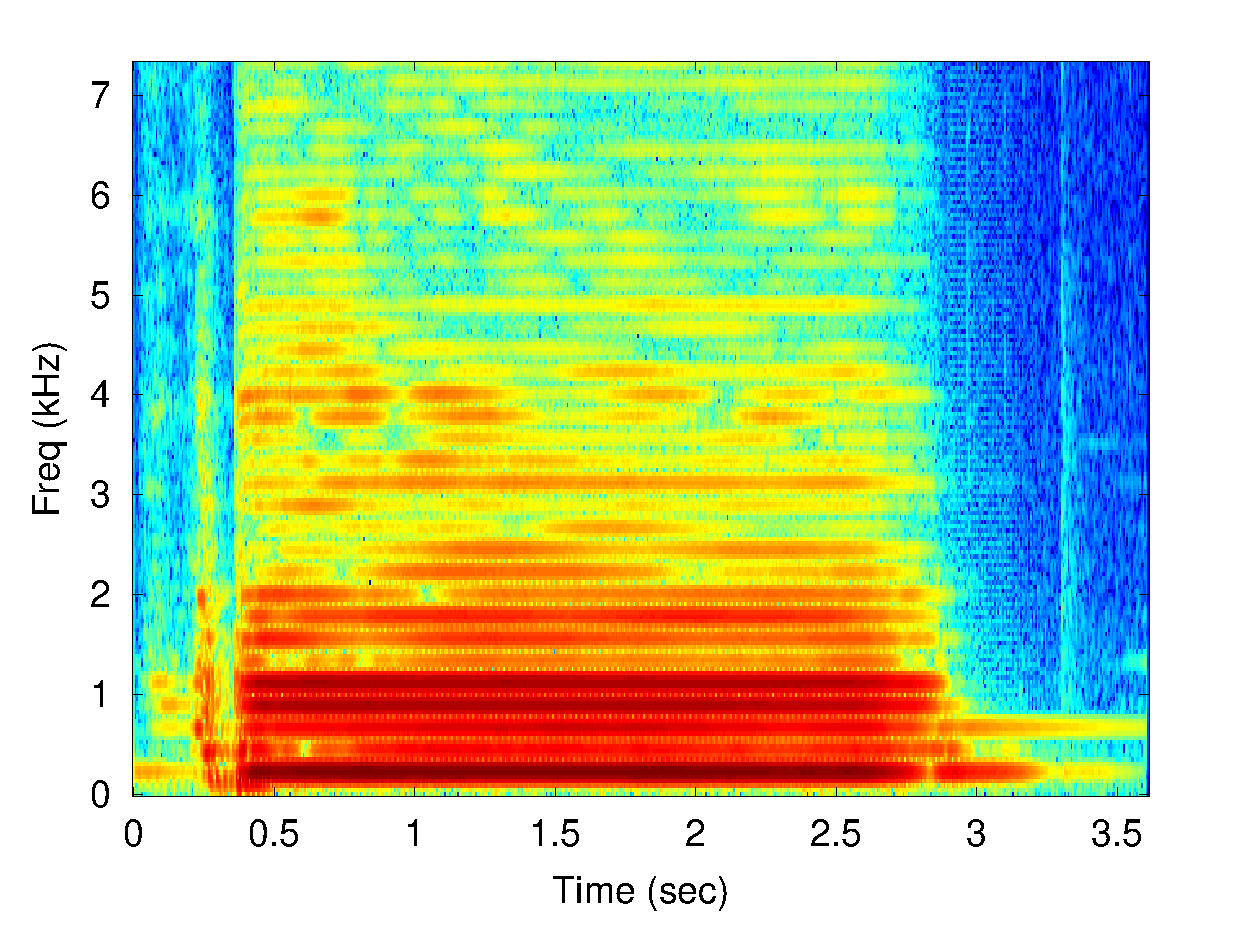
\includegraphics[width=0.45\textwidth]{chapter3/Images/CelloSpectrogram.eps}
				\label{fig:CelloSpectrogram}
			}
			\qquad
			\subfloat[Filtered Sample]
			{
				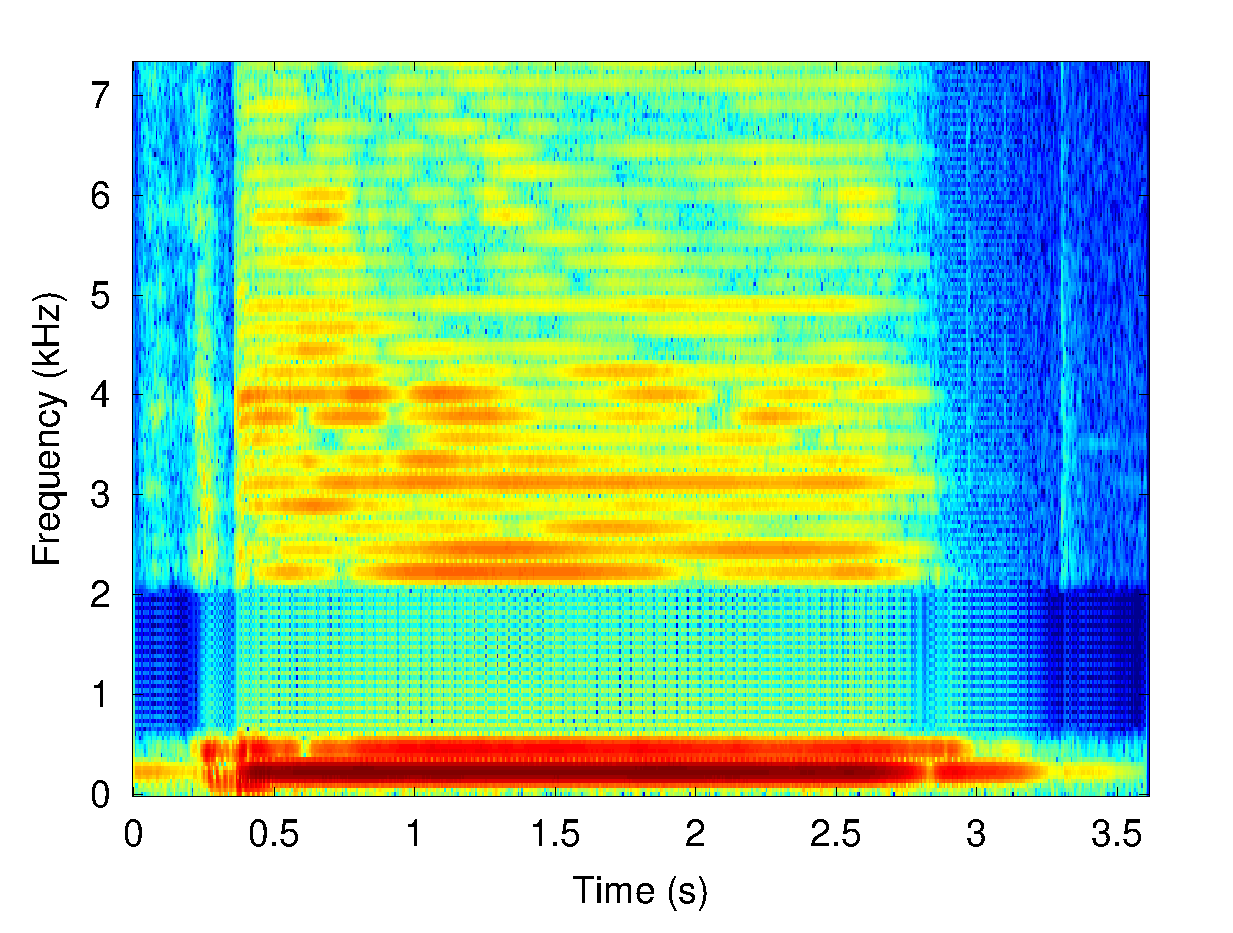
\includegraphics[width=0.45\textwidth]{chapter3/Images/CelloFilteredSpectrogram.eps}
				\label{fig:CelloFilteredSpectrogram}
			}
			\caption{Spectrograms of the cello sample.}
			\label{fig:CelloSpectrograms}
		\end{figure}

		Each sample was reconstructed three times using each method, using different parameters each time. For the
		SSBA and IAP methods a different order FIR filter was used to isolate the fundamental frequency. The
		filters used had orders of 50, 100 and 500. For the synthesis method the window length of the STFT was
		changed, taking values of 50, 100 and 500 samples. Spectrograms for the reconstructed samples using the
		smallest filter order / STFT window length are shown in Figure \ref{fig:ReconstructedCelloSpectrograms}.

		\begin{figure}[h!]
			\centering
			\subfloat[SSBA with a 50\super{th} order filter.]
			{
				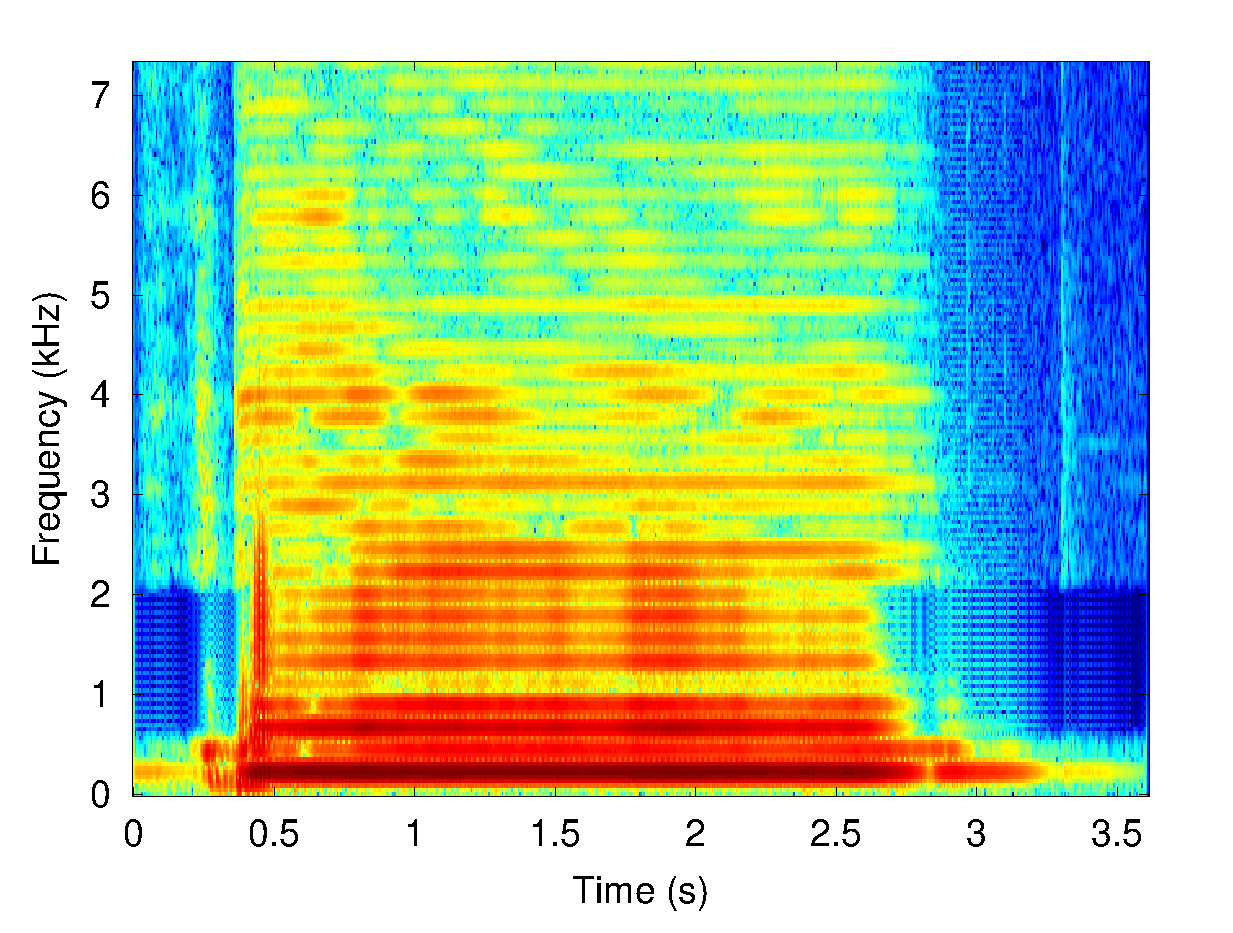
\includegraphics[width=0.45\textwidth]{chapter3/Images/CelloSSBASpectrogram.eps}
				\label{fig:CelloSSBASpectrogram}
			}
			\qquad
			\subfloat[IAP with a 50\super{th} order filter.]
			{
				\includegraphics[width=0.45\textwidth]{chapter3/Images/CelloIAPSpectrogram.eps}
				\label{fig:CelloIAPSpectrogram}
			}
			
			\subfloat[Synthesis with an STFT window length of 50 samples.]
			{
				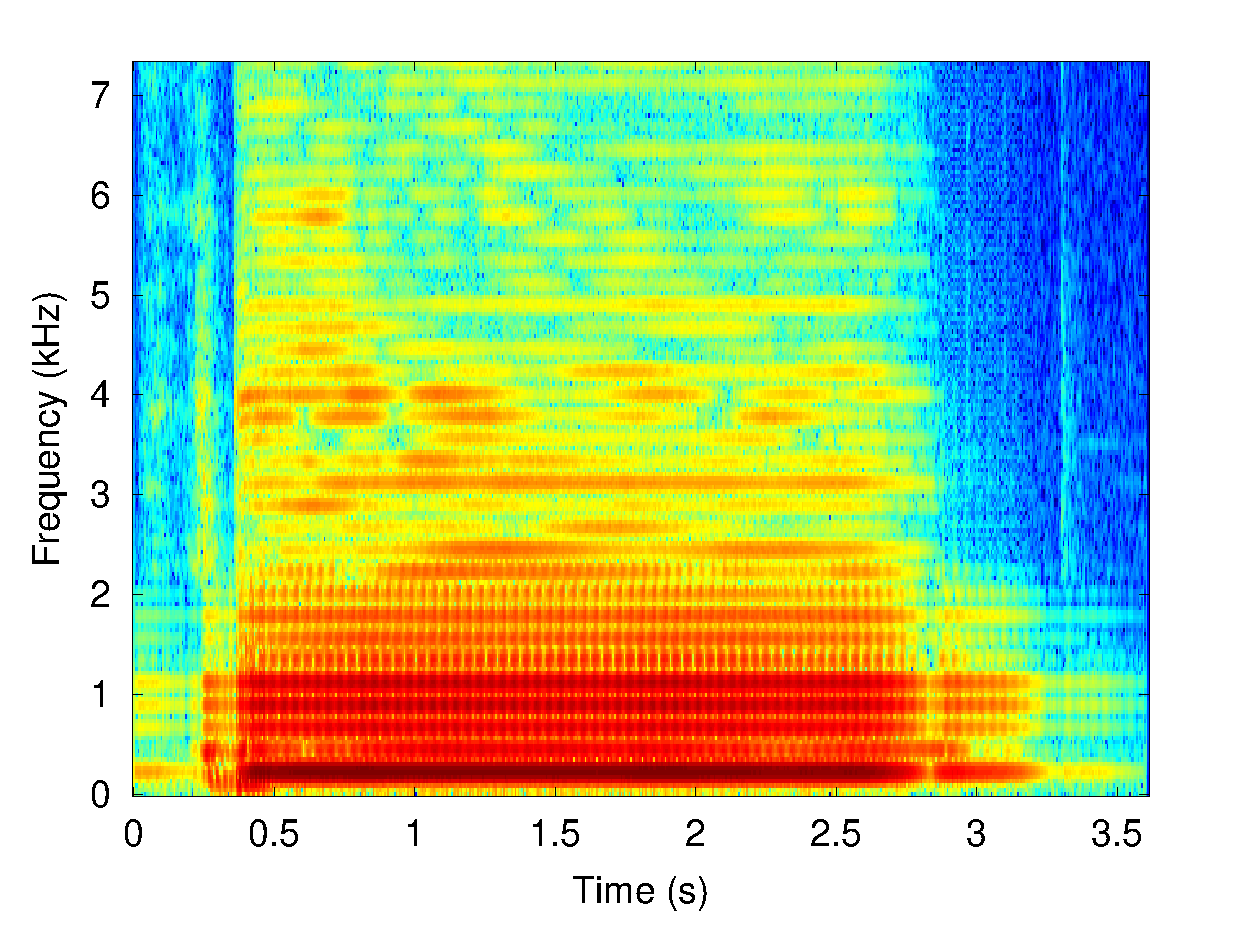
\includegraphics[width=0.45\textwidth]{chapter3/Images/CelloSynthesisSpectrogram.eps}
				\label{fig:CelloSynthesisSpectrogram}
			}
			\caption{Spectrograms of the cello sample reconstructed using three different methods.}
			\label{fig:ReconstructedCelloSpectrograms}
		\end{figure}

		On inspection of these spectrograms the characteristics of the three excitation methods can be seen. The
		amplitude envelopes of the generated harmonics differ greatly between the methods. Comparing the decay
		portion of the envelopes compared with those in the original signal (Figure \ref{fig:CelloSpectrogram})
		highlights these differences. In the cello sample the fundamental frequency and third harmonic have a
		longer decay time then the other harmonics. The harmonics generated by the IAP and synthesis methods
		(Figures \ref{fig:CelloIAPSpectrogram} and \ref{fig:CelloSynthesisSpectrogram}) use the amplitude envelope
		of the fundamental frequency extending the decay time of the these harmonics compared to that in the
		original. Those generated by the SSBA method (Figure \ref{fig:CelloSSBASpectrogram}) have shortened decay
		times. As the order of the harmonic is increased the decay time gets shorter due to the dynamic expansion
		shown in Figure \ref{fig:SSBATemporalEffects}.

		The amplitude envelopes of the harmonics generated using the synthesis techniques exhibit a large amount of
		ripple. This is due to the amplitude of the fundamental being calculated in blocks. These inaccuracies are
		not present in the harmonics generated using the IAP method as the amplitude is calculated on a sample by
		sample basis.

		Test participants were presented with all processed version of a particular sample at once along with a
		reference stimulus (the unprocessed sample) and an anchor stimulus (the sample with its harmonics removed).
		Participants were asked to grade how well each processed stimulus recreated the reference stimulus on a
		scale from 0 to 100.

		The results of this experiment are shown in Figure \ref{fig:SMCResults} with error bars showing the 95\%
		confidence intervals. The stimuli numbers refer to different processing algorithms as follows.

		\begin{tabular}{>{\bfseries}cl}
			1. & Reference Stimulus \\
			2. & Sample reconstructed using the synthesis method with an STFT window length of 50
			     samples. \\
			3. & Sample reconstructed using the synthesis method with an STFT window length of 100
			     samples. \\
			4. & Sample reconstructed using the synthesis method with an STFT window length of 500
			     samples. \\
			5. & Sample Reconstructed using the SSBA method using a 50\super{th} order filter.\\
			6. & Sample Reconstructed using the SSBA method using a 100\super{th} order filter.\\
			7. & Sample Reconstructed using the SSBA method using a 500\super{th} order filter.\\
			8. & Sample Reconstructed using the IAP method using a 50\super{th} order filter.\\
			9. & Sample Reconstructed using the IAP method using a 100\super{th} order filter.\\
		     	10. & Sample Reconstructed using the IAP method using a 500\super{th} order filter.\\
	     		11. & Sample with third through ninth harmonics removed (anchor).\\
		\end{tabular}

		\begin{figure}[h!]
			\centering
			\subfloat[Cello Sample]
			{
				\includegraphics[width=0.45\textwidth]{chapter3/Images/CelloResults.eps}
				\label{fig:CelloResults}
			}
			\qquad
			\subfloat[Clarinet Sample]
			{
				\includegraphics[width=0.45\textwidth]{chapter3/Images/ClarinetResults.eps}
				\label{fig:ClarinetResults}
			}

			\subfloat[Synthesised Sample]
			{
				\includegraphics[width=0.45\textwidth]{chapter3/Images/SynthResults.eps}
				\label{fig:SynthResults}
			}
			\qquad
			\subfloat[Piano Sample]
			{
				\includegraphics[width=0.45\textwidth]{chapter3/Images/PianoResults.eps}
				\label{fig:PianoResults}
			}
			\caption{Mean grades and confidence intervals for each of the stimuli.}
			\label{fig:SMCResults}
		\end{figure}

		Across all the samples there is a general increase in the perceived quality of the reproduction as the
		filter order or STFT window length is increased. With the SSBA and IAP methods increasing the filter order
		increases the level difference between the fundamental and its harmonics, better isolating the fundamental.
		This is turn reduces the levels of intermodulation distortion in the output producing a `cleaner' harmonic.
		With the synthesis method increasing the STFT window length increases the frequency resolution allowing for
		the amplitude envelope of the fundamental frequency to be measured more precisely.

		The piano sample used had very little energy at its fundamental frequency. This illustrates the problem
		discussed previously, there is not enough information in the amplitude envelope of the fundamental to
		reproduce the other harmonics. This leads to much lower grades for the reproduced signals than for any of
		the other samples. Figure \ref{fig:PianoResults} shows that the piano sample with its harmonics
		missing received a higher grade on average then any of the reconstructed samples further showing how poor
		the quality of the reconstructions is.

		The confidence intervals for the grades given to the majority of the stimuli are high. This is most likely
		due to there being too few participants in the experiment. To supplement these results each of the stimuli
		was graded with the R\sub{nonlin} metric. These results were normalised to the same range as the results
		from the listening test and are displayed in Figure \ref{fig:SMCRNonlin}.

		\begin{figure}[h!]
			\centering
			\subfloat[Cello Sample]
			{
				\includegraphics[width=0.45\textwidth]{chapter3/Images/CelloRNonlin.eps}
				\label{fig:CelloRNonlin}
			}
			\qquad
			\subfloat[Clarinet Sample]
			{
				\includegraphics[width=0.45\textwidth]{chapter3/Images/ClarinetRNonlin.eps}
				\label{fig:ClarinetRNonlin}
			}

			\subfloat[Synthesised Sample]
			{
				\includegraphics[width=0.45\textwidth]{chapter3/Images/SynthRNonlin.eps}
				\label{fig:SynthRNonlin}
			}
			\qquad
			\subfloat[Piano Sample]
			{
				\includegraphics[width=0.45\textwidth]{chapter3/Images/PianoRNonlin.eps}
				\label{fig:PianoRNonlin}
			}
			\caption{R\sub{nonlin} values for each of the stimuli.}
			\label{fig:SMCRNonlin}
		\end{figure}

		The R\sub{nonlin} values support the correlations found in the listening test results. Using a higher order
		filter to isolate the fundamental improves the quality of the reconstruction. Figure \ref{fig:PianoRNonlin}
		again illustrates the problems which arise when the input signal has little energy at its fundamental
		frequency. Several of the reconstructions are objectively less similar to the original signal than the
		anchor stimulus.

		Both sets of results show that, using the highest order filter / STFT window lengths, each of the methods
		produce similar quality reconstructions of the original signal. For shorter filter lengths the IAP method
		provides more quality at then the SSBA method at the expense of requiring slightly more computation. The
		synthesis method produces similar quality results but incurs further computational complexity. 
		
		For timbral control applications the IAP method provides the greatest flexibility. For the majority of
		stimuli in this experiment it reproduced signals with the highest perceived quality. It was also shown in
		section \ref{sec:FeatureControl-IAP} that it is a homogeneous process allowing it to be applied to a wider
		range of signals with more predictable effects.

\section{Controlling features with Exciters}
\label{sec:FeatureControl-Control}
